\section{Motivation} \label{sec:motivation}

In this section we make the argument for a more powerful function merging
approach. Consider the examples from two SPEC CPU2006 benchmarks shown in
Figures~\ref{fig:sphinx-example} and \ref{fig:libquantum-example}.

\begin{figure}[t!]
  \centering
  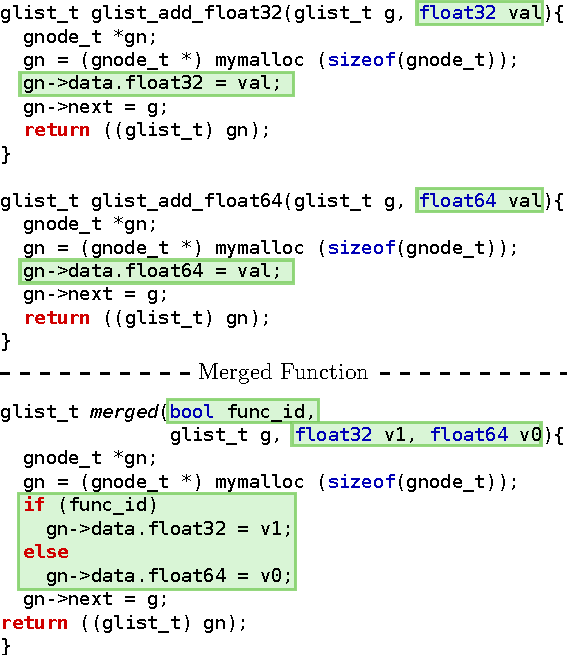
\includegraphics[width=.95\linewidth]{figs/sphinx-example.pdf}
  \caption{Example of two functions from the benchmark \texttt{sphinx} with
	different parameters that could be merged, as shown at the bottom.
    We highlight where they differ.}
  \label{fig:sphinx-example}
\end{figure}

Figure~\ref{fig:sphinx-example} shows two functions from the
\texttt{482.sphinx3} benchmark. The two functions are almost identical, only
their function arguments are of different types, \textit{float32} and
\textit{float64}, causing a single operation to be different. As shown at the
bottom of Figure~\ref{fig:sphinx-example}, these functions can be easily merged
in three steps. First, we expand the function argument list to include the
two parameters of different types. Then, we add a function identifier,
\texttt{func\_id}, to indicate which of the two functions is called. Finally,
we place the lines that are unique to one of the functions in an if-then-else, with
\texttt{func\_id} being the predicate. Overall, merging these two functions
reduces the total number of machine instructions by 18\%.

Despite being so similar, neither GCC or LLVM can merge the two functions.
They can only handle identical functions and functions where type mismatches
can be removed by lossless bitcasting of the conflicting variables. Similarly, the
state-of-the-art~\cite{edler14}, while much more powerful, cannot merge the two
functions either. It requires both functions to have the same list of parameters.

\begin{figure}[t!]
  \centering
  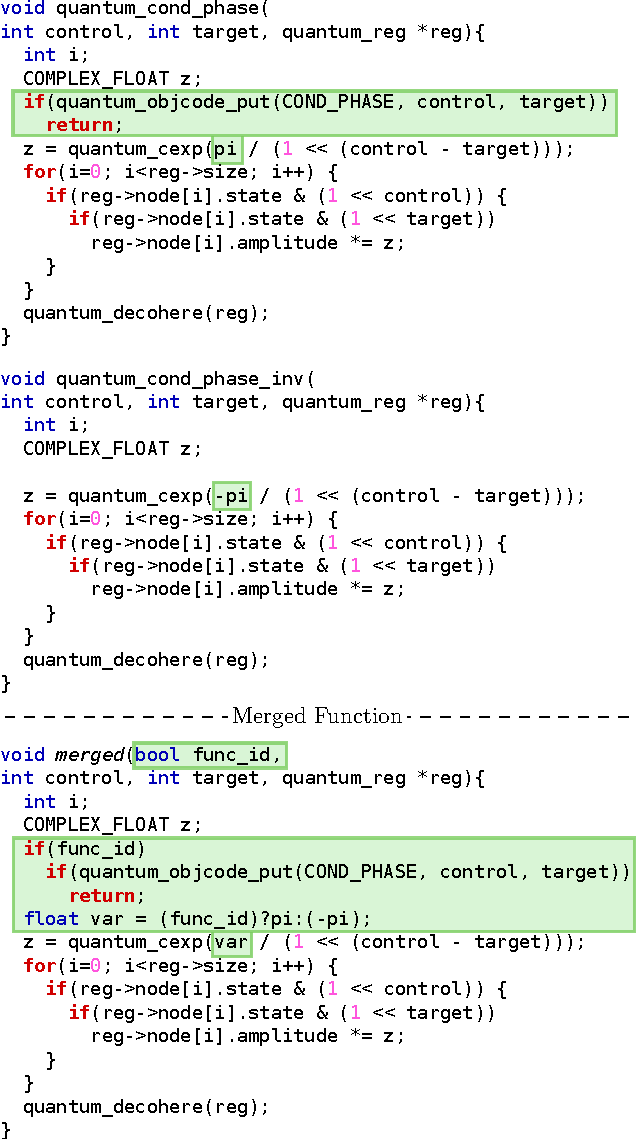
\includegraphics[width=\linewidth]{figs/libquantum-example.pdf}
    \caption{Example of two functions from the benchmark \texttt{libquantum}
	  with different CFGs that could be merged, as shown at the bottom.
      We highlight where they differ.}
  \label{fig:libquantum-example}
\end{figure}

Figure~\ref{fig:libquantum-example} gives another two functions extracted from \texttt{462.libquantum}. While these two functions have the
same signature, i.e. the same return type and list of parameters, they differ slightly in their bodies. Merging them manually
is straightforward, shown at the bottom of Figure~\ref{fig:libquantum-example}, reducing the number of instructions by 23\%. But again,
none of the existing techniques can merge the two functions. The state-of-the-art can work with non-identical functions, but it needs
their CFGs to be identical. Even a single extra basic block, as in this case, makes merging impossible.

These examples show that all existing techniques are severely limited.
Optimization passes in production compilers work only on effectively identical
functions. State-of-the-art techniques can merge functions only when they are
structurally similar, with identical signatures and isomorphic CFGs. All of
them miss massive opportunities for code size reduction. In the next sections,
we show a superior approach which removes such constraints and is able to merge
arbitrary functions, when it is profitable to do so.
